% -*-latex-*-
%\documentclass[handout]{beamer} 
\documentclass[12pt]{beamer} 
\usepackage{etex}

\let\latexput\put
\usepackage{pictex}
\let\pictexput\put
\let\put\latexput

\newcommand{\G}{\mathcal{G}}
\newcommand{\Het}{\mathcal{H}}
\newcommand{\mutation}{$\cdot$} 
\newcommand{\OR}{\;\hbox{or}\;}
\newcommand{\AND}{\;\&\;}
\usepackage{ifthen}
\newcounter{showthis}
\setcounter{showthis}{1}
\newdimen\thusfar
\newdimen\plotht
\newdimen\plotwd
\newdimen\plotsp
\newdimen\xunit
\newdimen\yunit
\newdimen\offsety
\setbeamercovered{transparent}
\begin{document}
\title{Drift When Populations Vary in Size}
\author{Alan R. Rogers}
\date{\today}
\frame{\titlepage}

\begin{frame}
\frametitle{Why is heterozygosity so often lower than we expect?}
\begin{itemize}
\item 
Urn model assumes $N$ is constant.  What if it varies?
\item 
Bottleneck: a temporary reduction in $N$
\item 
Decline in $\Het$ is faster than recovery.
\item 
Effective population size is harmonic mean of $N_t$
\item
Harmonic mean is sensitive to small sizes.
\end{itemize}
\end{frame}

\begin{frame}
\frametitle{A bottleneck in population size}
\begin{center}
\mbox{%
\sf
\beginpicture
\setcoordinatesystem units <0.0014\textwidth, 0.3\textheight> point at 0 0
\setplotarea x from 0 to 500, y from 0 to 1
%\plotheading{Population Size}
\axis left label {$2N$}
  ticks withvalues 100 5000 / at 0.02 1 / /
\axis bottom /
\plot 0 1 
      100 1
      100 0.02
      200 0.02
      200 1
      500 1 /
%%%%%%%%%%%%%%%%%%%%%%%%%%%%%%%%%%%%%%%%%%%%%%%%%%%%%%%%%%%%%%%%
\setcoordinatesystem units <0.0014\textwidth, 0.3\textheight> point at 0 1.2
\setplotarea x from 0 to 500, y from 0 to 1
%\plotheading{Gene Diversity}
\axis left label {$\mathcal{H}$}
  ticks withvalues 0.167 0.909 / at 0.167 0.909 / /
\axis bottom   label {Time in generations} 
  ticks numbered from 0 to 500 by 100 /
\setdots
\putrule from 0 0.167 to 500 0.167
\putrule from 0 0.909 to 500 0.909
\setsolid
\plot
0   0.9090909
100 0.9090909
110 0.8251379
120 0.7506783
130 0.6846385
140 0.6260665
150 0.5741177
160 0.5280433
170 0.4871790
180 0.4509356
190 0.4187906
200 0.3902806
210 0.4015697
220 0.4126133
230 0.4234165
240 0.4339847
250 0.4443229
260 0.4544361
270 0.4643293
280 0.4740072
290 0.4834745
300 0.4927358
310 0.5017956
320 0.5106583
330 0.5193281
340 0.5278092
350 0.5361058
360 0.5442219
370 0.5521614
380 0.5599281
390 0.5675258
400 0.5749581
410 0.5822288
420 0.5893412
430 0.5962989
440 0.6031052
450 0.6097634
460 0.6162767
470 0.6226482
480 0.6288812
490 0.6349785
500 0.6409431
/
\endpicture}
\end{center}

%%% Local Variables: 
%%% mode: latex
%%% TeX-master: t
%%% End: 

$\mathcal{H}$ declines rapidly, recovers slowly.  Why?
\end{frame}

\begin{frame}
\frametitle{What is a half-life?}
\mbox{%
\sf
\setbox0=\hbox{$\hat H$}
\beginpicture
%\valuestolabelleading=0.4\baselineskip
%\setcoordinatesystem units <0.017in, 2.5in>
\setcoordinatesystem units <0.003\textwidth, 0.5\textheight>
\setplotarea x from 0 to 231, y from 0 to 1
\axis left label {$H$}
  ticks numbered from 0 to 1 by 1 
        unlabeled at 0 0.1667 0.2708333 0.375 0.583333 1 /
        withvalues \box0 / at 0.1667 / /
\axis top label {Time in generations} 
  ticks withvalues 0 58 116 173 231 / at 0 58 116 173 231 / /
\axis bottom label {Half-lives} 
  ticks withvalues 0 1 2 3 4 / at 0 58 116 173 231 / /
\axis right /
\put {\small\begin{tabular}{r@{$\;=\;$}l}
  $u$ & 0.001\\
 $2N$ & 100
\end{tabular}} [rt] at 231 1

%Equilibrium heterozygosity
\setdashes
\plot 0 0.1667 231 0.1667 /
\setsolid
% hlife 1
\putrule from 0 0.5833333 to 58 0.5833333 
\putrule from 58 0.1667 to 58 0.5833333
% hlife 2
\putrule from 0 0.375 to 116 0.375 
\putrule from 116 0.375 to 116 0.1667
% hlife 3
\putrule from 0 0.2708333 to 173 0.2708333 
\putrule from 173 0.2708333 to 173 0.1667
% Heterozygosity
% 2N = 100.000000 u = 0.001000 theta = 0.200000 Heq = 0.166667 
% halfLife = 57.762265
%   t            H
\plot
    0    1.0000000
    6    0.9441942
   12    0.8921255
   17    0.8435437
   23    0.7982152
   29    0.7559223
   35    0.7164616
   40    0.6796435
   46    0.6452910
   52    0.6132389
%hlife 1 
%   t            H
   58    0.5833333
   64    0.5554304
   69    0.5293961
   75    0.5051052
   81    0.4824410
   87    0.4612945
   92    0.4415641
   98    0.4231551
  104    0.4059788
  110    0.3899528
%hlife 2 
%   t            H
  116    0.3750000
  121    0.3610485
  127    0.3480314
  133    0.3358859
  139    0.3245538
  144    0.3139806
  150    0.3041154
  156    0.2949109
  162    0.2863227
  168    0.2783097
%hlife 3 
%   t            H
  173    0.2708333
  179    0.2638576
  185    0.2573490
  191    0.2512763
  196    0.2456102
  202    0.2403236
  208    0.2353910
  214    0.2307888
  219    0.2264947
  225    0.2224882
%hlife 4 
%   t            H
  231    0.2187500
/
\endpicture}

\end{frame}

\begin{frame}
\frametitle{Why the decline is faster than the recovery}

\begin{columns}
\column{0.45\textwidth}
Gene diversity converges toward equilibrium with a half-life of
\[
t_h = \frac{\ln 2}{2u + 1/2N}
\]
Small $N$ $\Rightarrow$ short half-life.

\medskip

$N$ has little effect if $2u \gg 1/2N$, i.e.\ if $\theta \gg 1$.
\column{0.55\textwidth}
\begin{tabular}{crrr}
&&\multicolumn{2}{c}{Half-life of}\\
     && \multicolumn{2}{c}{convergence}\\ \cline{3-4}
$2N$ &$\theta$& \multicolumn{1}{c}{(gen.)} & (years)\\ \hline\hline
$\infty$ &$\infty$ & 347 & 1,041\\
$10^6$   &2000.00 &  346 & 1,038\\
$10^5$   &200.00 &  345 & 1,035\\
$10^4$   &20.00 &  330 &   990\\
$10^3$   &2.00 & 231 &   693\\
$10^2$   &0.20 &  58  &   174\\
$10$     &0.02 &   7  &    21\\
\hline
\multicolumn{3}{c}{(Assumes $u=0.001$)}
\end{tabular}
\end{columns}
\end{frame}

\begin{frame}
\frametitle{Oscillations in population size}

We've been considering a single bottleneck in population size. What if
it is always varying?

To see that this is plausible, consider the record of climate change
during the past 250,000 years.
\end{frame}

\begin{frame}
\frametitle{History of global temperature}
\begin{columns}
\column{0.65\textwidth}
\includegraphics[width=\textwidth]{grip.pdf}
\column{0.4\textwidth}
What did this do to population size?
\end{columns}
\end{frame}

\begin{frame}
\noindent\includegraphics[width=0.9\textwidth]{neigraur.png}\\
Heterozygosity, $\Het$, versus population size, $Ng$, where $g$ is
ploidy. Solid line: expected curve for neutral alleles; dotted:
slightly overdominant; dot-dashed: slightly deleterious.\\
\mbox{}\hfill\small (Nei \& Graur 1984)\\ 
\end{frame}

\begin{frame}
For many species, $\Het$ is much smaller than would be expected on the basis
of their population sizes.  Could this be a result of population size
bottlenecks during the Pleistocene?
\end{frame}

\begin{frame}
  \frametitle{Effective population size, $N_e$}

 Goal: Find a value of $N$ that makes our idealized population behave like a
 more complicated one.

 Example: In a randomly mating population of constant size, heterozygosity
 (gene diversity) is equal to
\[
\Het = \frac{4Nu}{4Nu+1}
\]
What if the population varies in size?
\end{frame}

\begin{frame}
\frametitle{Review: $\Het$ in a population of constant size}
\begin{eqnarray*}
  \Het_1 &=& \Het_{0} \left(1 - \frac{1}{2N}\right)\\
\end{eqnarray*}
\end{frame}

\begin{frame}
\frametitle{Another generation}
\begin{eqnarray*}
  \Het_1 &=& \Het_{0}\left(1 - \frac{1}{2N}\right)\\
  \Het_2 &=& \Het_{1}\left(1 - \frac{1}{2N}\right)\\
\end{eqnarray*}
\end{frame}

\begin{frame}
\begin{eqnarray*}
  \Het_1 &=& \Het_{0}\left(1 - \frac{1}{2N}\right)\\
  \Het_2 &=& \Het_{1}\left(1 - \frac{1}{2N}\right)\\
         &=& \Het_{0}\left(1 - \frac{1}{2N}\right)^2\\
\end{eqnarray*}
\end{frame}

\begin{frame}
\frametitle{General form}
\begin{eqnarray*}
  \Het_t &=& \Het_{0}\left(1 - \frac{1}{2N}\right)^t\\
         &\approx& \Het_{0} \exp[-t/2N]
\end{eqnarray*}

\bigskip

Note approximation: $1-x \approx e^{-x}$ when $x$ is small.
\end{frame}

\begin{frame}
\frametitle{$\Het$ in a population of varying size}
\begin{eqnarray*}
  \Het_1 &=& \Het_{0} \left(1 - \frac{1}{2N_0}\right)\\
\end{eqnarray*}
where $N_0$ is population size in generation~0.
\end{frame}

\begin{frame}
\frametitle{Another generation}
\begin{eqnarray*}
  \Het_1 &=& \Het_{0}\left(1 - \frac{1}{2N_0}\right)\\
  \Het_2 &=& \Het_{1}\left(1 - \frac{1}{2N_1}\right)\\
\end{eqnarray*}
\end{frame}

\begin{frame}
\frametitle{Two generations}
\begin{eqnarray*}
  \Het_2 &=& \Het_{0}\left(1 - \frac{1}{2N_0}\right)
                     \left(1 - \frac{1}{2N_1}\right)\\
\end{eqnarray*}
\end{frame}

\begin{frame}
\frametitle{Two generations again}
\begin{eqnarray*}
  \Het_2 &=& \Het_{0}\left(1 - \frac{1}{2N_0}\right)
                     \left(1 - \frac{1}{2N_1}\right)\\
 &=& \Het_{0} \prod_{i=0}^{1}\left(1 - \frac{1}{2N_{i}}\right)
\end{eqnarray*}

\bigskip

where $\prod$ is the product operator.
\end{frame}

\begin{frame}
\frametitle{General form}
\begin{eqnarray*}
  \Het_t &=& \Het_{0} \prod_{i=0}^{t}\left(1- \frac{1}{2N_{i}}\right)\\
  &\approx& \Het_{0}\exp\left[-\sum_{i=0}^{t-1}\frac{1}{2N_{i}}\right]
\end{eqnarray*}
\end{frame}

\ifthenelse{\theshowthis=0}{%
\begin{frame}
\frametitle{Approximation}
\begin{eqnarray*}
  \Het_t &=& \Het_{0} \prod_{i=0}^{t}\left(1 - \frac{1}{2N_{i}}\right)\\
  &\approx& \Het_{0} \prod_{i=0}^{t-1}\exp[-1/2N_{i}]\\
\end{eqnarray*}

\bigskip

How do you simplify a product of exponentials?
\end{frame}

\begin{frame}
\frametitle{Remember rule for product of exponentials}
\[
e^a e^b = \exp[a + b]
\]
\end{frame}

\begin{frame}
\frametitle{Product of exponentials is exponential of sum}
\begin{eqnarray*}
  \Het_t &\approx& \Het_{0} \prod_{i=0}^{t-1}\exp[-1/2N_{i}]\\
  &=& \Het_{0}\exp\left[-\sum_{i=0}^{t-1}\frac{1}{2N_{i}}\right]
\end{eqnarray*}
\end{frame}
}{}

\begin{frame}
\frametitle{Compare results for fixed and varying $N$}
\[
\begin{array}{rclrcl}
  \multicolumn{3}{c}{\hbox{Fixed $N$}} &
  \multicolumn{3}{c}{\hbox{Varying $N$}}\\
  \Het_t &\approx& \Het_{0} \exp[-t/2N_e]
  &&=&\Het_{0} \exp\left[-\sum_{i=0}^{t-1}\frac{1}{2N_{i}}\right]
\end{array}
\]
\begin{itemize}
\item
$N_e$ is called effective population size.
\item It is the constant population size that makes the two sides equal.
\end{itemize}
\end{frame}

\begin{frame}
The two sides are equal when
\[
1/N_e = \frac{1}{t}\sum_{i=0}^{t-1}\frac{1}{N_{i}}
\]
The effective population size, $N_e$, is the ``harmonic mean'' of $N_0, N_1,
\ldots, N_{t-1}$.
\end{frame}

\begin{frame}
  \frametitle{What is $N_e$ good for?}

In a population of varying size, average heterozygosity at neutral
loci is
\[
\Het = \frac{4N_eu}{4N_eu+1}
\]
where $N_e$ is the effective population size.
\end{frame}

\begin{frame}
\frametitle{Example}
\begin{itemize}
\item
What is the arithmetic mean of 1, 50, and 100?
\item
What is the harmonic mean?
\end{itemize}
\end{frame}

\begin{frame}
\frametitle{Answer}
\begin{itemize}
\item
Arithmetic mean: $(1 + 50 + 100)/3 = 50.3333$.
\item
Harmonic mean: $1/((1 + 1/50 + 1/100)/3) = 2.9126$.
\end{itemize}
Harmonic mean is \emph{much} smaller than arithmetic mean.\\
\end{frame}

\begin{frame}
\frametitle{Approach toward equilibrium when size varies}
{\centering\setbox0=\hbox{$\searrow$}
\setbox1=\hbox{$\hat H(N_e)$}
\setbox2=\hbox{\raise\ht0\box1\box0}
\mbox{%
\beginpicture
%%%%%%% Top Plot %%%%%%%%
\setcoordinatesystem units <0.0005\textwidth, 0.005\textheight> point at 0 0
\setplotarea x from -500 to 1000, y from 0 to 50
% y-axis measured in units of 100
\axis left label {$2N$}
  ticks withvalues 100 5000 / at 1 50 / /
\axis bottom   %label {Time in generations} 
  ticks numbered from 0 to 900 by 300 /
%Effective population size
\put {\raise \ht0 \hbox{$2N_e$}$\searrow$} [rb] at -100 1.96
\setdashes
\plot -100 1.96 990 1.96 /
%Population size
\setsolid
  \plot
    -500  50
    0     50
%epoch  0
%   t         2N
    0     1
  100     1
%epoch  1       
%   t         2N
  100    50
  200    50
%epoch  2       
%   t         2N
  200     1
  300     1
%epoch  3       
%   t         2N
  300    50
  400    50
%epoch  4       
%   t         2N
  400     1
  500     1
%epoch  5       
%   t         2N
  500    50
  600    50
%epoch  6       
%   t         2N
  600     1
  700     1
%epoch  7       
%   t         2N
  700    50
  800    50
%epoch  8       
%   t         2N
  800     1
  900     1
%epoch  9       
%   t         2N
  900    50
  990    50
/
%%%%%%% Bottom Plot %%%%%%%%
\setcoordinatesystem units <0.0005\textwidth, 0.25\textheight> point at 0 1.5
\setplotarea x from -500 to 1000, y from 0 to 1
\axis left label {$H$}
  ticks numbered from 0.0 to 1.0 by  0.5 /
\axis bottom   label {Time in generations} 
  ticks numbered from 0 to 900 by 300 /
%Equilibrium heterozygosity
\put {\box2} [rb] at 0 0.281690
\setdashes
\plot 0 0.281690 990 0.281690 /
\setsolid
%Heterozygosity
  \plot
   -500   0.9090909 
%epoch  0
   0  0.9090909
  10  0.8251379
  20  0.7506783
  30  0.6846385
  40  0.6260665
  50  0.5741177
  60  0.5280433
  70  0.4871790
  80  0.4509356
  90  0.4187906
%epoch  1
 100  0.3902806
 110  0.4015697
 120  0.4126133
 130  0.4234165
 140  0.4339847
 150  0.4443229
 160  0.4544361
 170  0.4643293
 180  0.4740072
 190  0.4834745
%epoch  2
 200  0.4927358
 210  0.4558641
 220  0.4231618
 230  0.3941574
 240  0.3684329
 250  0.3456172
 260  0.3253816
 270  0.3074342
 280  0.2915162
 290  0.2773983
%epoch  3
 300  0.2648768
 310  0.2788948
 320  0.2926077
 330  0.3060222
 340  0.3191448
 350  0.3319819
 360  0.3445397
 370  0.3568242
 380  0.3688414
 390  0.3805971
%epoch  4
 400  0.3920970
 410  0.3666054
 420  0.3439964
 430  0.3239441
 440  0.3061592
 450  0.2903855
 460  0.2763954
 470  0.2639873
 480  0.2529823
 490  0.2432218
%epoch  5
 500  0.2345650
 510  0.2492425
 520  0.2636006
 530  0.2776464
 540  0.2913864
 550  0.3048276
 560  0.3179762
 570  0.3308387
 580  0.3434213
 590  0.3557302
%epoch  6
 600  0.3677712
 610  0.3450304
 620  0.3248611
 630  0.3069725
 640  0.2911068
 650  0.2770352
 660  0.2645547
 670  0.2534856
 680  0.2436681
 690  0.2349609
%epoch  7
 700  0.2272382
 710  0.2420751
 720  0.2565892
 730  0.2707875
 740  0.2846769
 750  0.2982640
 760  0.3115554
 770  0.3245576
 780  0.3372769
 790  0.3497195
%epoch  8
 800  0.3618913
 810  0.3398154
 820  0.3202358
 830  0.3028703
 840  0.2874684
 850  0.2738082
 860  0.2616927
 870  0.2509472
 880  0.2414168
 890  0.2329641
%epoch  9
 900  0.2254672
 910  0.2403427
 920  0.2548945
 930  0.2691296
 940  0.2830551
 950  0.2966774
 960  0.3100034
 970  0.3230394
 980  0.3357918
 990  0.3482666
/
\endpicture}
\\}
\end{frame}


\title{Genetics and the History of Population Size}
\author{Alan R. Rogers}
\date{\today}
\frame{\titlepage}

\begin{frame}
\frametitle{Mismatch Distributions of Amerindian mtDNA Haplogroups}
\begin{columns}
\column{0.7\textwidth}
\includegraphics[height=0.8\textheight]{fagundesmm.png}
\column{0.3\textwidth}
\footnotesize Fagundes et al 2008
\end{columns}
\end{frame}

\begin{frame}
\frametitle{Genealogies of Amerindian mtDNA Haplogroups}
\centering
\includegraphics[width=0.9\textwidth]{fagundestree.png}%
\llap{\footnotesize Fagundes et al 2008}\\
\end{frame}

\begin{frame}
\frametitle{Estimated Size of Amerindian Population}
\includegraphics[width=0.9\textwidth]{fagundespop.png}%
\llap{\footnotesize Fagundes et al 2008}\\
\end{frame}

\begin{frame}
\frametitle{Estimated Size of Bison Population}
\includegraphics[width=0.9\textwidth]{bison.jpeg}
\end{frame}

\begin{frame}
\frametitle{What about the nuclear genome}

\begin{itemize}
\item Huge amounts of data.
\item Recombination makes previous methods unusable.
\end{itemize}
\end{frame}

\ifthenelse{\theshowthis=0}{
\begin{frame}
\frametitle{Deep History}
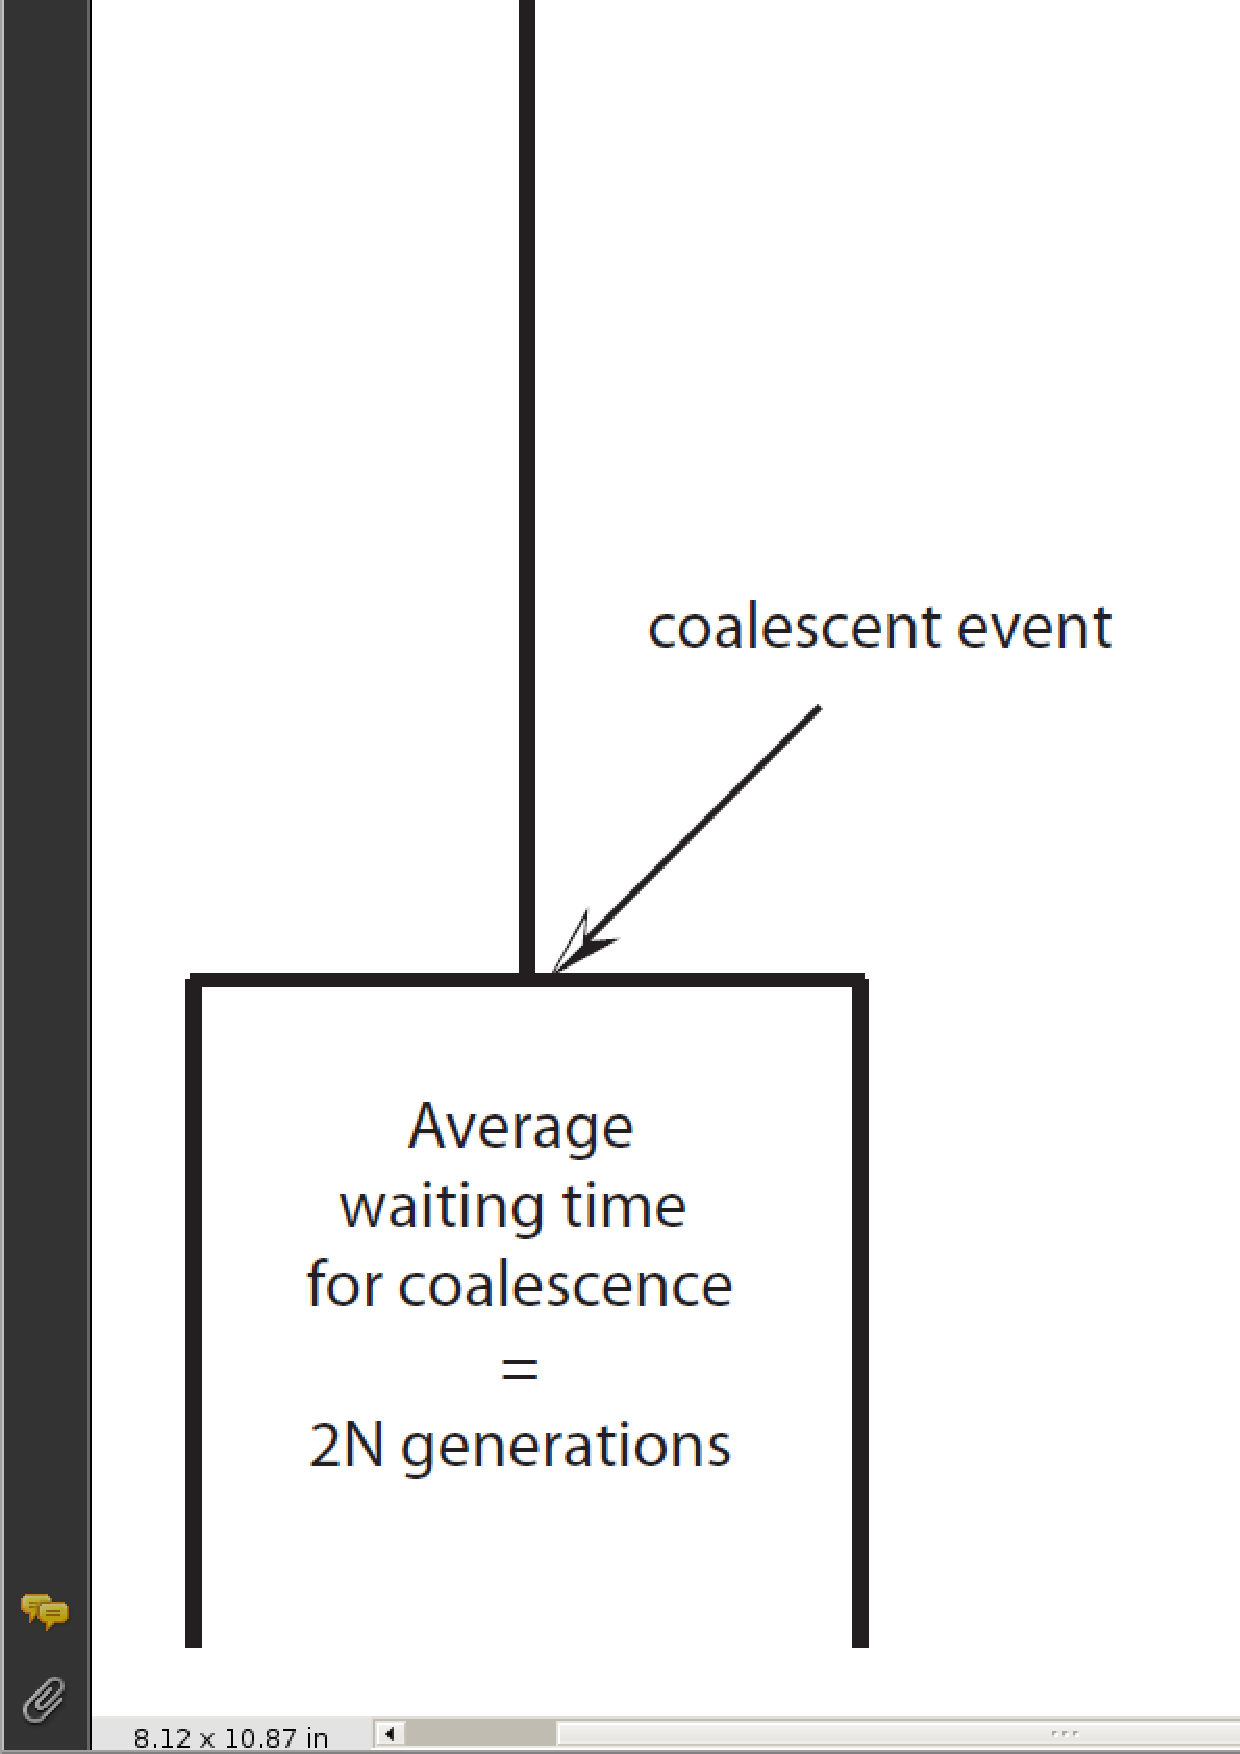
\includegraphics[height=0.8\textheight]{Huff-deeptree.png}
\footnotesize Huff et al 2010
\end{frame}

\begin{frame}
\frametitle{Deep History}
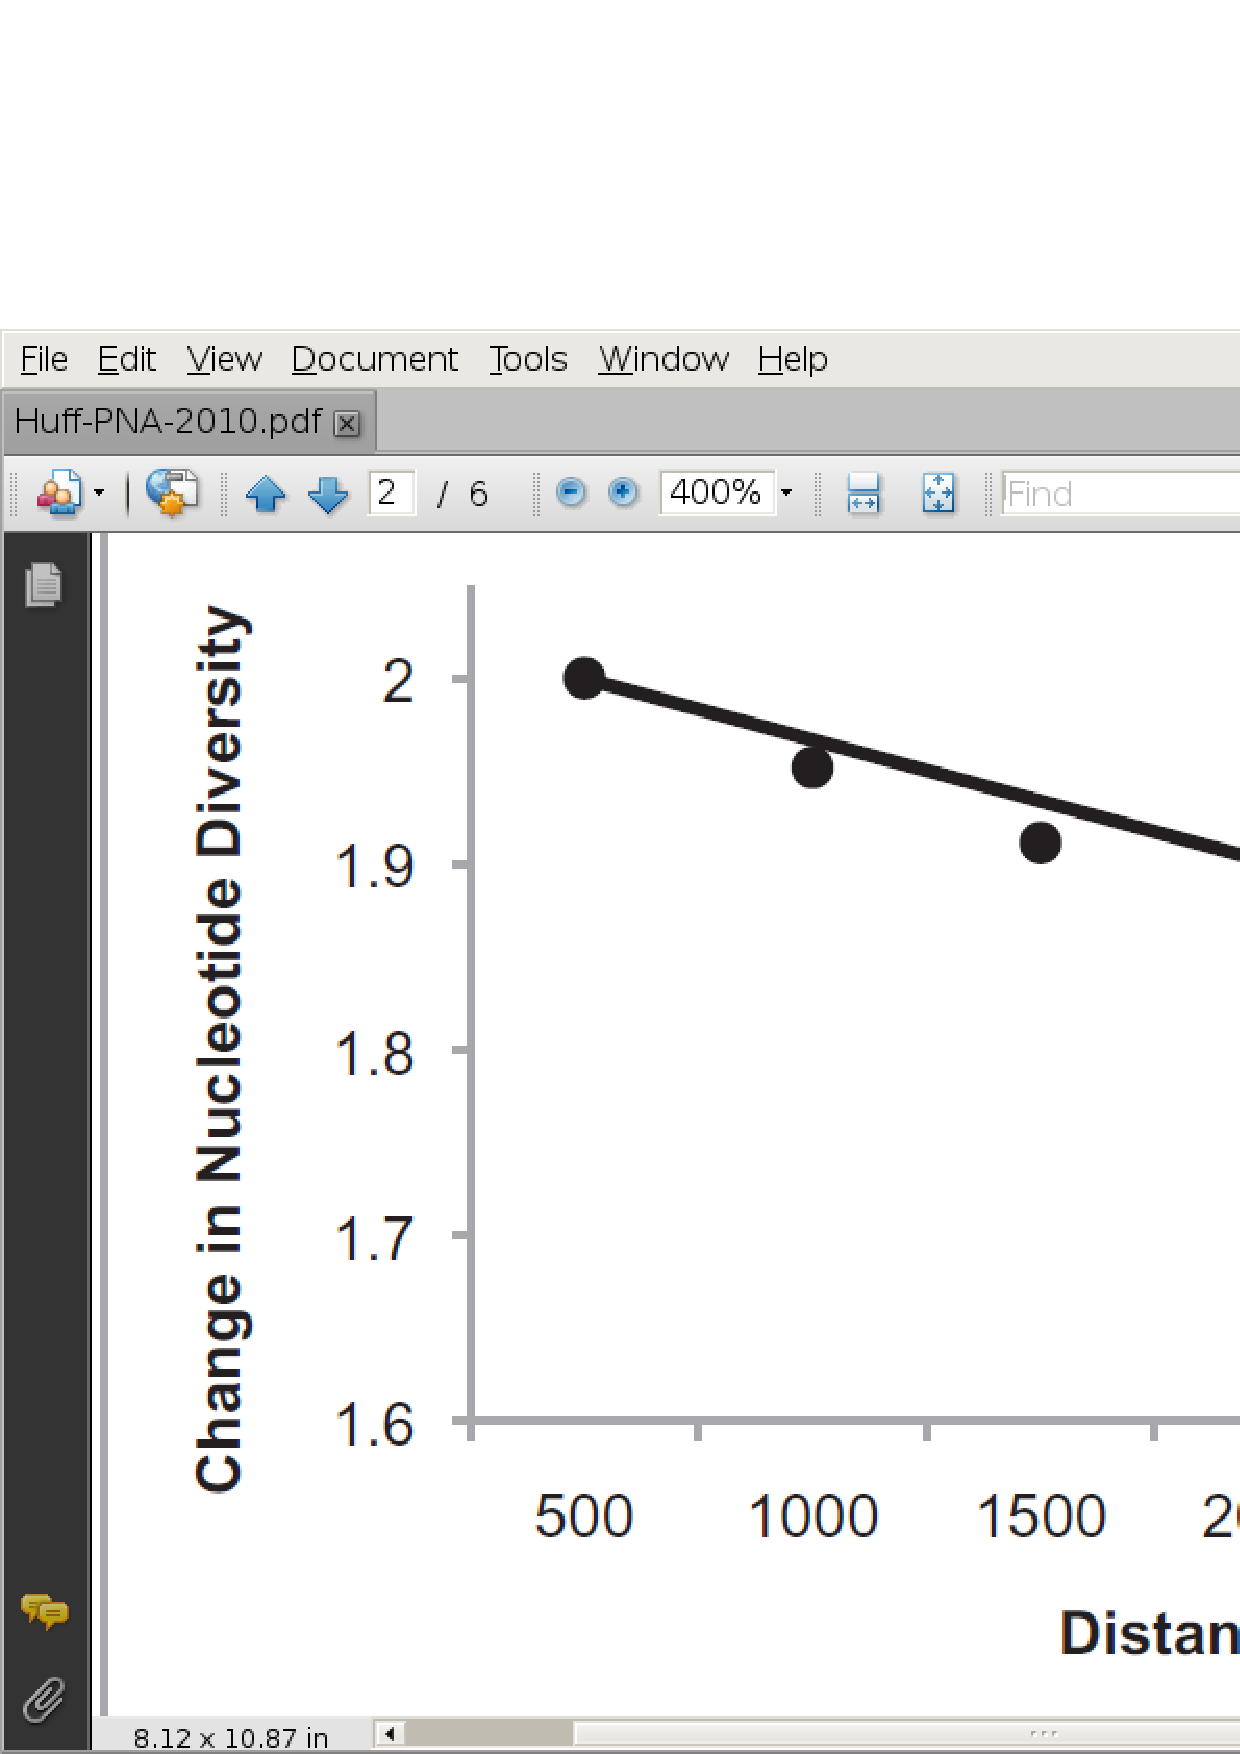
\includegraphics[width=\textwidth]{Huff-scatter.png}\\
\mbox{}\hfill\footnotesize Huff et al 2010
\end{frame}

\begin{frame}
\frametitle{Deep History}
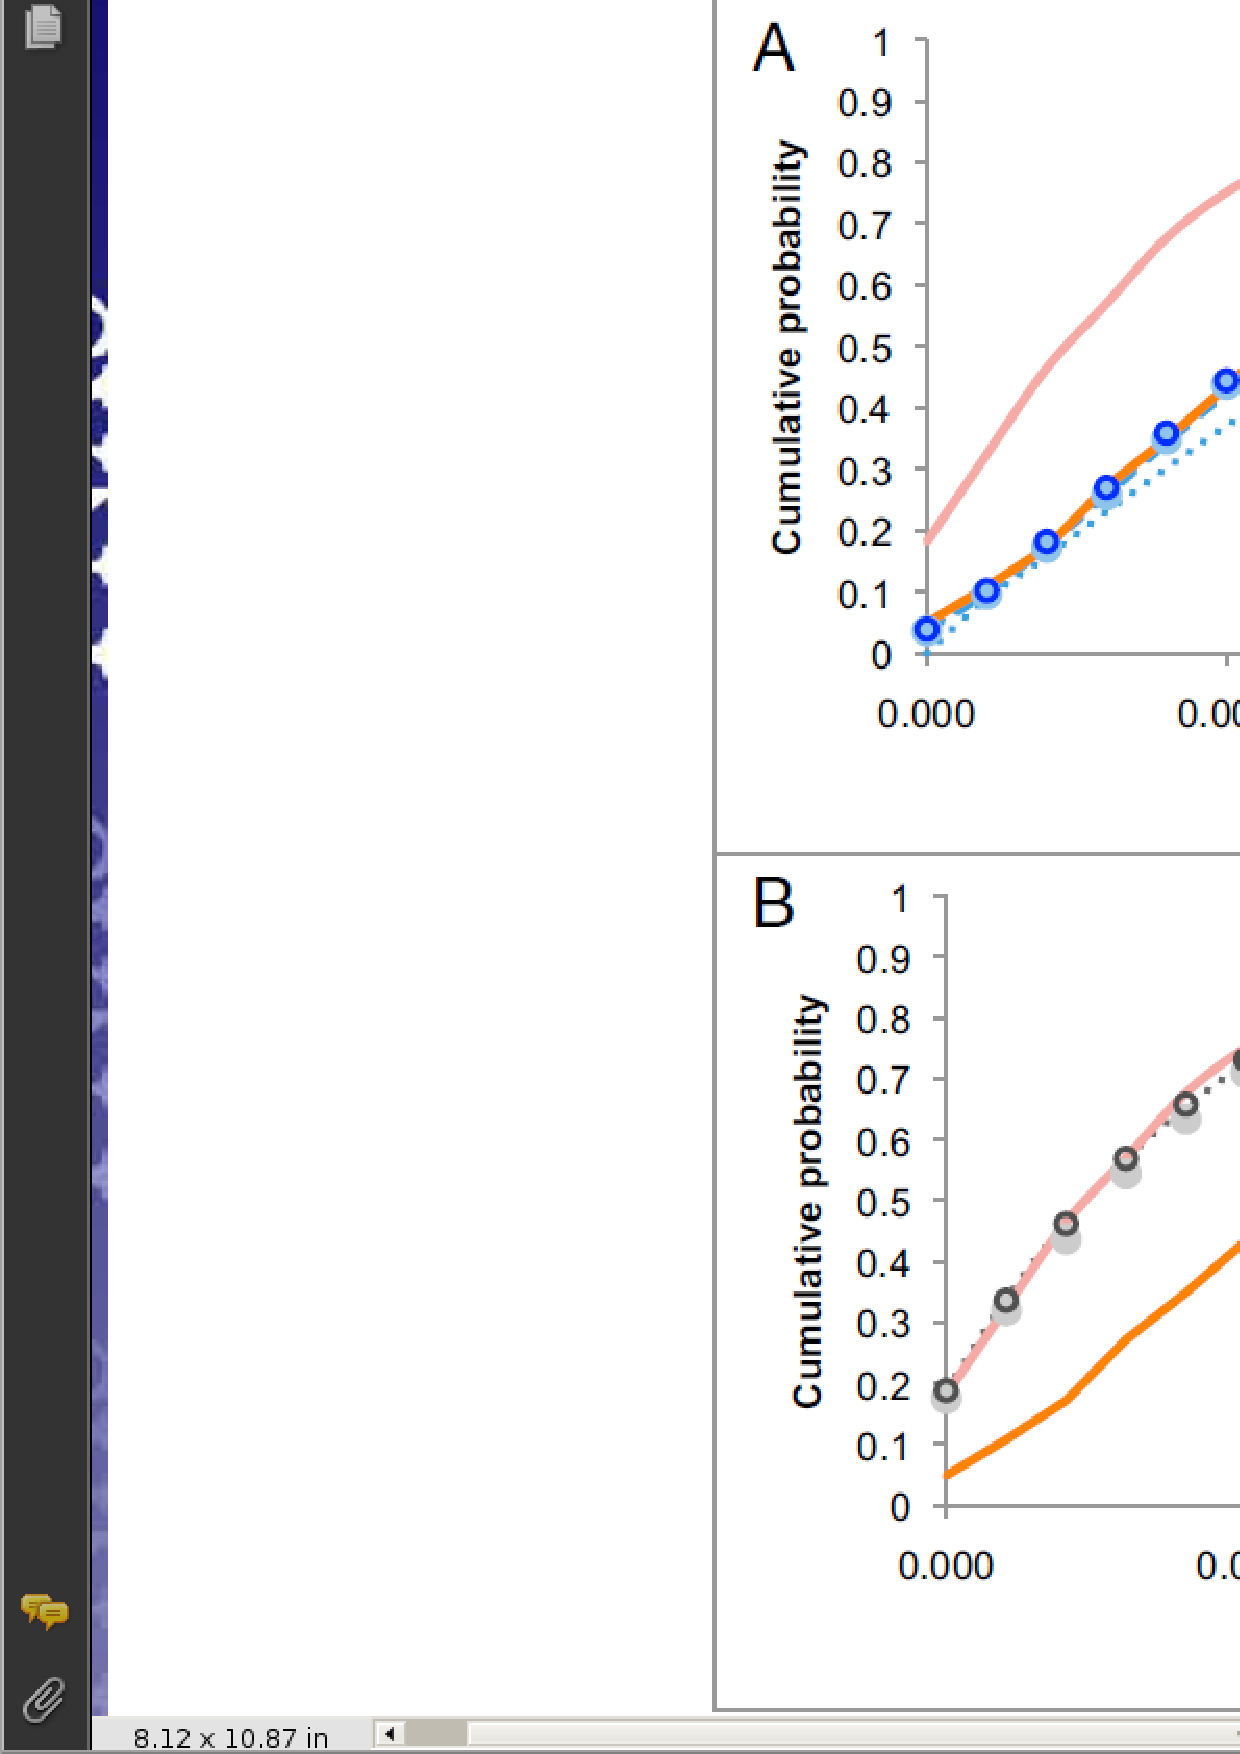
\includegraphics[height=0.8\textheight]{Huff-cumprob.png}\\
\mbox{}\hfill\footnotesize Huff et al 2010
\end{frame}

\begin{frame}
\frametitle{Deep History}
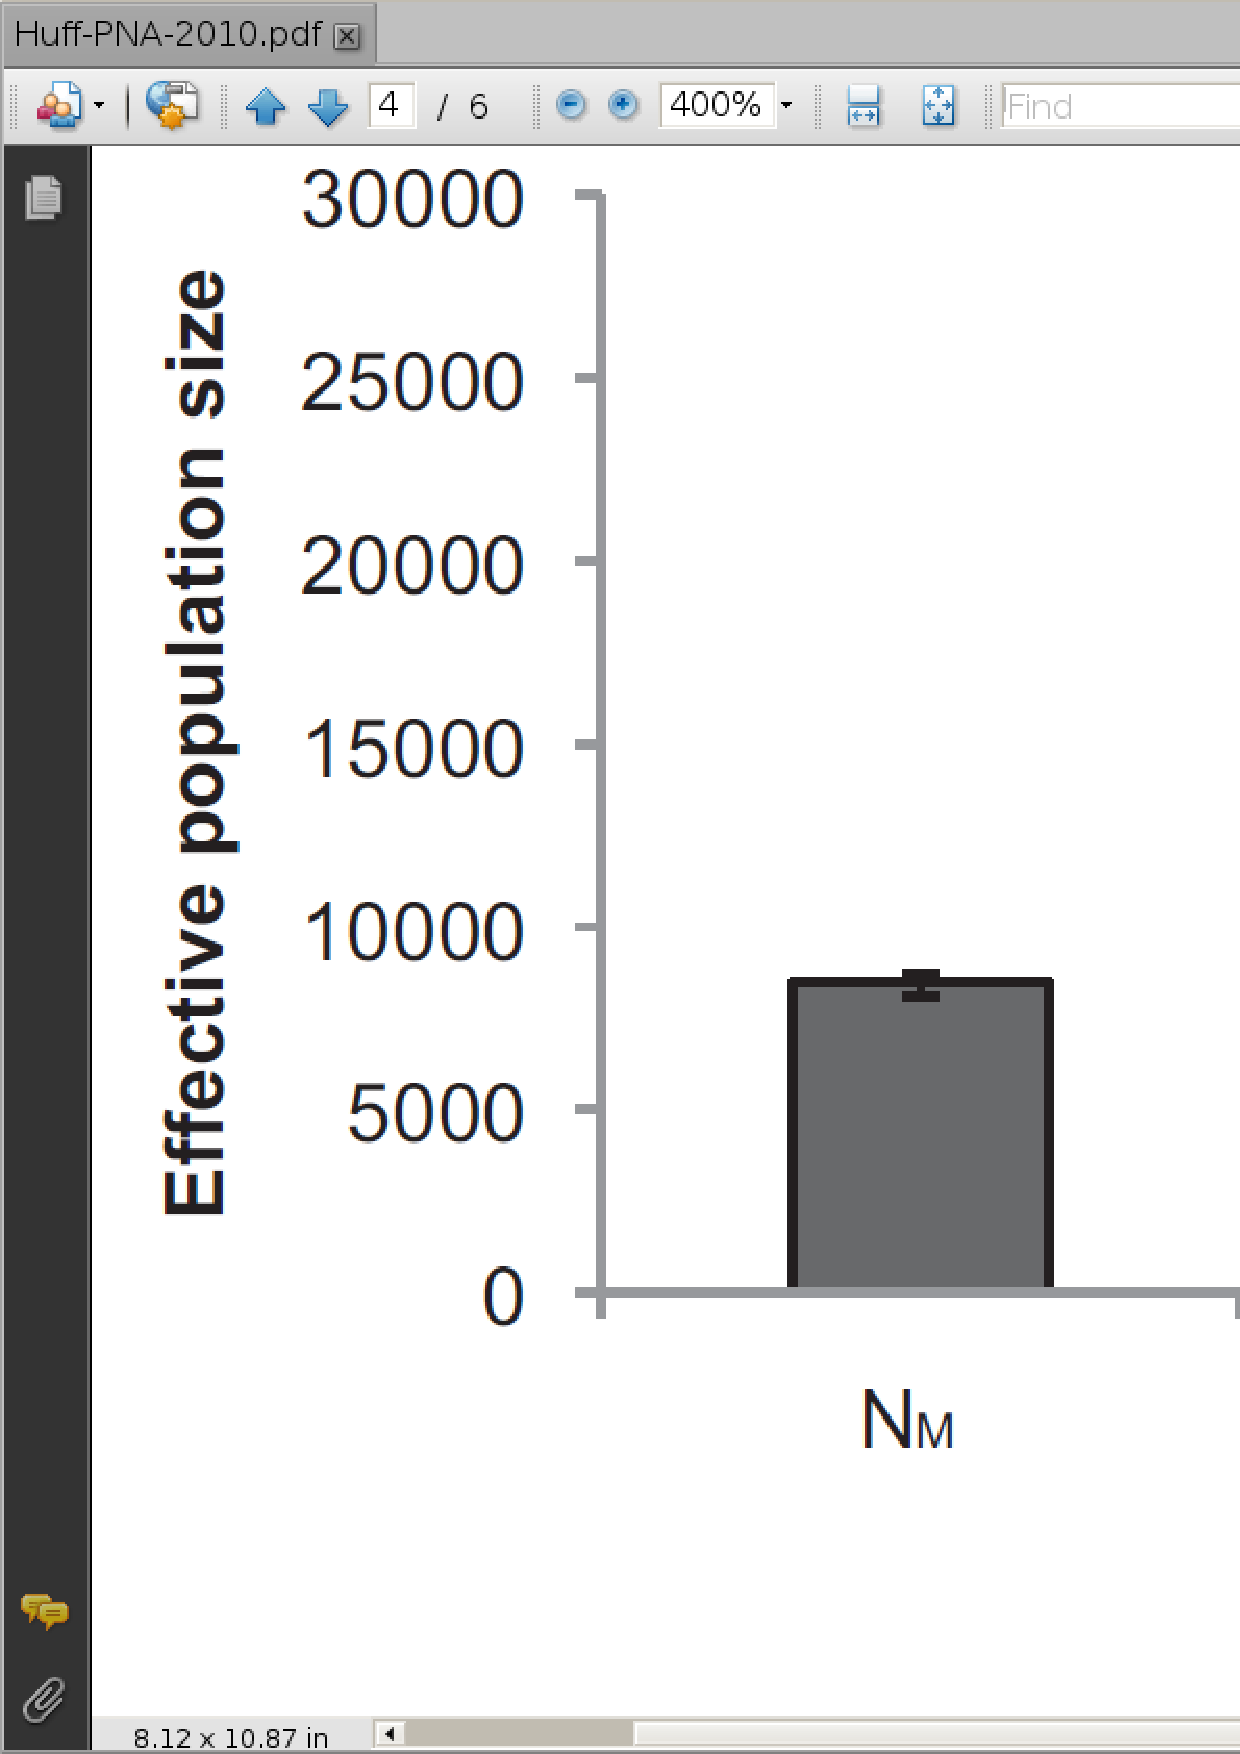
\includegraphics[width=\textwidth]{Huff-estimates.png}\\
\mbox{}\hfill\footnotesize Huff et al 2010
\end{frame}
}{}

\begin{frame}
\frametitle{PSMC: deep history from a single diploid genome}
\includegraphics[width=\textwidth]{prufer-pophist.jpg}\\[-2ex]
{\mbox{}\hfill\footnotesize Pr{\"u}fer et al 2014}

Accurate back to 2~mya. Not for last 20,000 years.
\end{frame}%

\begin{frame}
\begin{columns}
\column{0.7\textwidth}
\includegraphics[width=\linewidth]{stairway.png}
\column{0.35\textwidth}
\raggedleft
\textcolor{blue}{\large Stairway plot}

\bigskip

Uses site frequency spectrum.

\bigskip

Accomodates large samples. Can study last 20,000 years.

\bigskip

Liu \& Fu 2015
\end{columns}
\end{frame}

\begin{frame}
\frametitle{SMC++}
\includegraphics[width=\textwidth]{Terhorst-smcpp.png}\\

\small 8 modern populations and Ust'-Ishim (45-kya modern Siberian). Log
scale on left, arithmetic on right.  Combines advantages of PSMC and
spectrum. Large samples or small; accurate across both recent and deep
scales of time. (Terhorst et al. 2017)
\end{frame}

%\begin{frame}
\frametitle{Population tree}
\centering%-*-latex-*-
\let\put\pictexput
\mbox{\beginpicture
\headingtoplotskip=\baselineskip
\setcoordinatesystem units <4mm, 4mm> point at 16 1
\setplotarea x from 1 to 15, y from 1 to 15
\small
\axis bottom invisible ticks length <0pt>
  withvalues {$X$} {$Y$} {$N$} {$D$} /  at 2 7 10 14 / /
%\axis bottom invisible shiftedto y=-0.3 ticks length <0pt>
%  withvalues {$x$} {$y$} {$n$} {$d$} /  at 2 7 10 14 / /
\axis left invisible ticks length <0pt>
  withvalues {$T_{XY}$} {$T_{XYND}$} /
   at 4 11.249724127083585 / /
\axis right invisible ticks length <0pt>
  withvalues {$T_{ND}$}  / at 6 / /
\put {\small Pops:} [r] <0pt, 3pt> at 1 0
%\put {\small Samples:} [rt] <0pt, -4pt> at 1 -0.3
\setdots
\putrule from 1 4 to 4.5 4   % $T_{XY}$
\putrule from 12 6 to 15 6 % $T_{ND}$
%\putrule from 12.75 2 to 15.75 2 % $T_D$
\putrule from 1 11.249724127083585
   to 8.12486206354179 11.249724127083585 % $T_{XYND}$
\setsolid
\setplotsymbol ({\normalsize .})
\plot 1 1 7 13 7 15 /   %X
\plot 3 1 4.5 4 6 1 /   %XY
\plot 8 1 5.5 6 8.12486206354179 11.249724127083585 /    %Y
\plot 9.17572 1 10.1757 6 11.036 7.7206 / %N
\plot 11 1 12 6 /       %N
\plot 13 1 12 6 /            %D
\plot 14.684 1 13.8151 6 12.3389 8.9523 9 13 9 15 / %Dr
\plot 8.12486206354179 11.249724127083585 11.036 7.7206 / % ND l
\arrow <10pt> [.2,.67] from 9.57571931984138 3 to 7 3
%\arrow <0pt> [.2,.67] from 12.75 2 to 11.25 2
%\arrow <10pt> [.2,.67] from 9.32572 2 to 7.5 2
\put {\small $N_{XY}$} at 6 9
\put {\small $N_{ND}$} at 11.2 9
\put {\small $N_N$}   at 10.7 4.3
\put {\small $N_{XYND}$} [b] <0pt,2pt> at 8 15
\put {\small $\alpha$} [b]  <0pt,5pt> at 8.5 3
%\put {\small $\epsilon$} [t]  <0pt,-5pt> at 12 2
\endpicture}
\let\put\latexput
\\[1ex]
$X$, Africa; $Y$, Europe; $N$, Neanderthal; $D$, Denisovan\\
\end{frame}

\begin{frame}
\frametitle{Gene genealogies and nucleotide site patterns}
\begin{columns}
\column{0.6\textwidth}
\centering\input{../pophist/figgptree}\\[1ex]
\column{0.4\textwidth}
\raggedleft
Gene genealogy within population tree.

\bigskip

Mutation on red branch $\rightarrow$ \emph{site pattern} \textcolor{red}{$yn$}.

\bigskip

Blue branch $\rightarrow$ \textcolor{blue}{$ynd$}.

\bigskip

0, ancestral; 1, derived.
\end{columns}
\end{frame}

\begin{frame}
\frametitle{Observed Site Pattern Frequencies}
\begin{columns}
\column{0.6\textwidth}
\includegraphics[width=\linewidth]{../pophist/patfrq.pdf}\\

\medskip

\centering
(fraction of nucleotide sites exhibiting each pattern)\\
\column{0.4\textwidth}
\raggedleft
$X$, Africa; $Y$, Europe; $N$, Neanderthal; $D$, Denisovan.

\bigskip

$xy$ is common because $X$ and $Y$ share ancestry.

\bigskip

Ditto $nd$.

\bigskip

Goal: infer history from these data
\end{columns}
\end{frame}

\begin{frame}{The mystery of the 4000-year-old Denisovan}
     We argued in 2017 for an early separation of Neanderthals and
     Denisivans and a bottleneck among their ancestors. Mafessoni and
     Pr{\"u}fer showed that results are different if one includes
     singleton site patterns. However, the with-singleton anaysis also
     implied an implausible 4~kya date for the Denisovan fossil. How
     can this be explained?
\end{frame}

\begin{frame}{Clues: an excess of site patterns $d$ and $xyn$}
     {\centering\includegraphics[width=\linewidth]{../pophist/singleton.pdf}\\
       \includegraphics[width=\linewidth]{../pophist/triplet.pdf}\\} Suggests
     hyperarchaic admixture into Denisovans (Pr\"{u}fer et al.\ 2014)
     or early modern admixture into Neanderthals (Kuhlwilm et al.\
     2016).
\end{frame}


\begin{frame}
\frametitle{Two ways to inflate $d$ and $xyn$.}
{\centering\input{../pophist/fighyparch}~%auto-ignore
%-*-latex-*-
\mbox{\beginpicture
\headingtoplotskip=0.2\baselineskip
\setcoordinatesystem units <2mm, 1.8mm>
\setplotarea x from -2 to 17.5, y from 0 to 20
\color{black}
\plotheading{$XY{\rightarrow}N$}
\axis bottom invisible ticks length <0pt>
  withvalues {$X$} {$Y$} {$N$} {$D$} {$H$} /  at 1 6 9 13 17 / /
\color{red}
\axis bottom invisible shiftedto y=-2.5 ticks length <0pt>
  withvalues {\llap{$d$:}} {0} {0} {0} {1} /
  at 0 1 6 9 13 / /
\color{cyan}
\axis bottom invisible shiftedto y=-5 ticks length <0pt>
  withvalues {\llap{$xyn$:}} {1} {1} {1} {0} /
  at 0 1 6 9 13 / /
\color{black} % I issue this command twice, because otherwise,
\color{black} % the rest of the document is cyan.
%\axis left ticks andacross numbered from 0 to 20 by 2 /
%\axis top ticks andacross numbered from 0 to 16 by 2 /
\setplotsymbol ({\normalsize .})
\plot 0 0 6 12 6 20 /   %X
\plot 2 0 3.5 3 5 0 /   %XY
\plot 7 0 4.5 5 7.12486206354179 10.249724127083585 /    %Y
\plot 8.17572 0 9.1757 5 10.036 6.7206 / %N
\plot 10 0 11 5 /       %N
\plot 12 0 11 5 /            %Dl
\plot 8 16 14.21226360816738 8.468963009740001 15.684 0 / %Hl
\plot 8 20 8 18.8112 15.8936 9.24189 17.4997 0 / %Hr
\plot 13.684 0 12.8151 5 11.3389 7.9523 8 12 8 16 / %Dr
\plot 7.12486206354179 10.249724127083585 10.036 6.7206 / % ND l
%\arrow <10pt> [.2,.67] from 8.57571931984138 2 to 6 2
%\arrow <0pt> [.2,.67] from 11.75 1 to 10.25 1
%\arrow <10pt> [.2,.67] from 8.32572 1 to 6.5 1
%\put {\small $m_N$} [b]  <0pt,5pt> at 7.5 2
%\put {\small $m_D$} [t]  <0pt,-5pt> at 11 1
\put {\small $m_{XY}$} [b]  <0pt,5pt> at 7.3 6
\arrow <10pt> [.2,.67] from 5 6 to 9.6 6
%\put {\small $m_H$} [b]  <0pt,5pt> at 13.9889 4
%\arrow <10pt> [.2,.67] from 14.9889 4 to 12.9889 4
\setplotsymbol ({\footnotesize .})
\setdashes
\plot 1 0 5 8 /         % x, bottom of xy
\setplotsymbol ({\textcolor{cyan}{\footnotesize .}})
\setsolid
\plot 5 8 7 12 7 13 /  % top of xy
\setplotsymbol ({\footnotesize .})
\setdashes
\plot 7 13 7 20 /             % top of xynd
\plot 6 0 4 4 4 6 / %y
\setplotsymbol ({\textcolor{red}{\footnotesize .}})
\setsolid
\plot
   12.649562539059012 0.5
   11.946500312472102 4
   10.581012916966557 7.465564584832791
   7.31003 11.4308
   7 13
/ % d and nd
\setplotsymbol ({\footnotesize .})
\setdashes
\plot
   9.187899999999999 0.5
   10.287899999999999 6
   5 6
   5 8
   / % n
\setsolid
\endpicture}
\\}
\textcolor{red}{Red} branch mutations generate site pattern $d$;
\textcolor{cyan}{Blue} generates $xyn$; 0, ancestral allele; 1,
derived; $X$, Africa; $Y$, Eurasia; $N$, Neanderthal; $D$,
Denisovan; $H$, Hyperarchaic; $XY$, population ancestral to $X$
and $Y$.
\end{frame}

\begin{frame}
\begin{raggedleft}
\includegraphics[width=0.8\linewidth]{../pophist/french-ma-mdot.pdf}\\
\includegraphics[width=0.83\linewidth]{../pophist/french-ma-tdot.pdf}\\
\includegraphics[width=0.83\linewidth]{../pophist/french-ma-ndot.pdf}\\
\end{raggedleft}
\end{frame}

\begin{frame}
\frametitle{Implications of previous slide}
   \begin{tabular}{lp{0.8\linewidth}}
   $m_H$, $T_{XYNDH}$ & \raggedright Substantial
     $H{\rightarrow}D$ admixture and a hyperarchaic separation time of
     $\sim$1.6~mya.\tabularnewline
   $m_{XY}$ & \raggedright $XY{\rightarrow}N$ admixture.\tabularnewline
   $T_{ND}$ & \raggedright Early separation of Neanderthals and Denisovans:
   $\sim$747~kya.\tabularnewline
   $2N_{ND}$ & \raggedright Narrow bottleneck in Neanderthal-Denisovan
   ancestors.\tabularnewline
   $2N_{AV}$, $2N_N$ & \raggedright Effective Neanderthal population was large
     early ($2N_{AV}\approx 21$~k) but small later ($2N_N\approx
     5$~k).\tabularnewline
   $T_V$, $T_A$, $T_D$ & \raggedright Vindija, Altai, and Denisovan fossil
     ages are $\sim$70~ky, $\sim$150~ky, and $\sim$100~ky.\tabularnewline
   \end{tabular}
\end{frame}

\begin{frame}
\frametitle{Summary (part 1)}
\begin{itemize}
\item History of population size affects depth of gene trees, genetic
  variation, and length of MRCA segments.
\item We can use these facts to infer the history of population size.
\item Human population has varied in size over past 3~my.
\item Bottleneck during last ice age, ending 20~kya.
\item African bottleneck was shorter and shallower.
\item Eurasian/African split 150~kya.
\item European/Asian split 20~kya.
\end{itemize}
\end{frame}

\begin{frame}
\frametitle{Summary (part 2)}

\textbf{Current consensus}
\begin{itemize}
\item Neanderthals and Denisovans separated $\sim$450 kya,
\item then declined to tiny population sizes ($<$1000 individuals).
\end{itemize}

\bigskip

\textbf{Our view}
\begin{itemize}
\item Archaics separated from moderns 750~kya,
\item then endured a bottleneck of $\sim$5~ky.
\item Neanderthals \& Denisovan separated shortly thereafter.
\item Neanderthal population was large early \& small later.
\end{itemize}
\end{frame}

\end{document}
